The signal is characterized by high \MET, no isolated leptons, and a CA15 jet identified as a Higgs boson candidate. In the signal region (SR) described
below, the dominant background contributions arise from Z+jets, W+jets, and \ttbar production. To model these processes data events in different control regions (CR) are used: single-lepton CRs are designed to constrain the \ttbar and W +jets backgrounds, while dilepton CRs constrain the Z+jets background contribution. The hadronic recoil $U$ defined by removing the \pt of the lepton(s) from the \MET computation in CRs is used as proxy for the \MET distribution of the main background processes in SR. 

Events are selected online by requiring large \MET.
% (to be greater than thresholds of $90$, $100$, $110$, or $120\GeV$) and large $H_{\mathrm{T}}^{\mathrm{miss}}$. Online \MET is calculated as the magnitude of the negative vectorial sum of the \pt of all particles at the trigger level and $H_{\mathrm{T}}^{\mathrm{miss}}$ is defined as the magnitude of the vectorial sum of the \pt of all jets in the event with 
%$p_{\mathrm{T}}>20\GeV$. 
The identified muons are not used in the \MET calculation performed online.
Additional events selected by requiring high-\pt single electrons are used to populate the CRs. 
%Thresholds imposed online on the electron \pt vary from 25\,GeV to 105\,GeV depending on the identification and isolation criteria.  

Offline events are selected requiring \MET ($U$) to be larger than 200~\GeV in the SR (CRs). A single CA15 jet with \pt greater than 200~\GeV and $|\eta|<2.4$ is required as the Higgs boson candidate. Appropriate requirements on its mass and its $N_2$ are placed in order to identify it as a $\mathrm{H}\to\mathrm{b}\bar{\mathrm{b}}$-tagged jet.
 
Multijet events can act as a source of background when the energy of at least one of the jets is mismeasured. 
Therefore, the absolute difference between the azimuthal angles of the vector \ptvecmiss\ and any other AK4 jet with $\pt>30~\GeV$ 
is required to be $>0.4$\,rad. 

The event preselection described above is common for the SR and all the CRs. The preselected events are split into different SR and CRs based on their lepton multiplicity and the presence of a narrow b tagged AK4 jet non overlapping with the Higgs candidate CA15 jet.
% Table~\ref{tab:event_selection} summarizes the differents requirements that define the SR and the CRs. 

%\begin{table}
%  \begin{center}
%  \caption{Event selection used to separate SR and CRs. This selection is applied on top of the preselection common to all regions, 
%as described in the text. } \label{tab:event_selection}
%    \begin{tabular}{  l | c | c | c  }
%      \hline \hline
%        region   & additional AK4 b tag   & leptons & double-b tag \\ \hline
%        signal   & 0                & 0       & pass \\ \hline
%        \ttbar   & 1                & 1       & pass/fail\\ \hline
%        W        & 0                & 1       & pass/fail\\ \hline
%        Dilepton & 0                & 2       & pass/fail\\
%      \hline \hline
%    \end{tabular}
%  \end{center}
%\end{table}


For the SR, events are rejected if they have any isolated electrons (muons) with $\pt >10\GeV$ and $|\eta|< 2.5$ (2.4) or 
any $\tau_\mathrm{had}$ candidates with $\pt > 18$\GeV and $|\eta|<2.3$~\cite{Khachatryan:2015hwa,Chatrchyan:2013sba,CMSTauJINST}. The events are further required to have no good quality photon with $\pt> 15$\GeV and $|\eta|<2.5$. An additional requirement on double-b tagger output of the selected Higgs boson candidate CA15 jet is placed.
To reduce the contamination from top quark pair production, the events must not have any additional AK4 b-tagged jets or more than one additional AK4 jet.
Figure \ref{Fig_cr_Recoil_fail} shows the expected \MET distribution in the the SR for all the expected SM backgrounds with \cPZpr-2HDM model signal hypothesis overlaid on it. 

\begin{figure}
\centering
 \subfloat{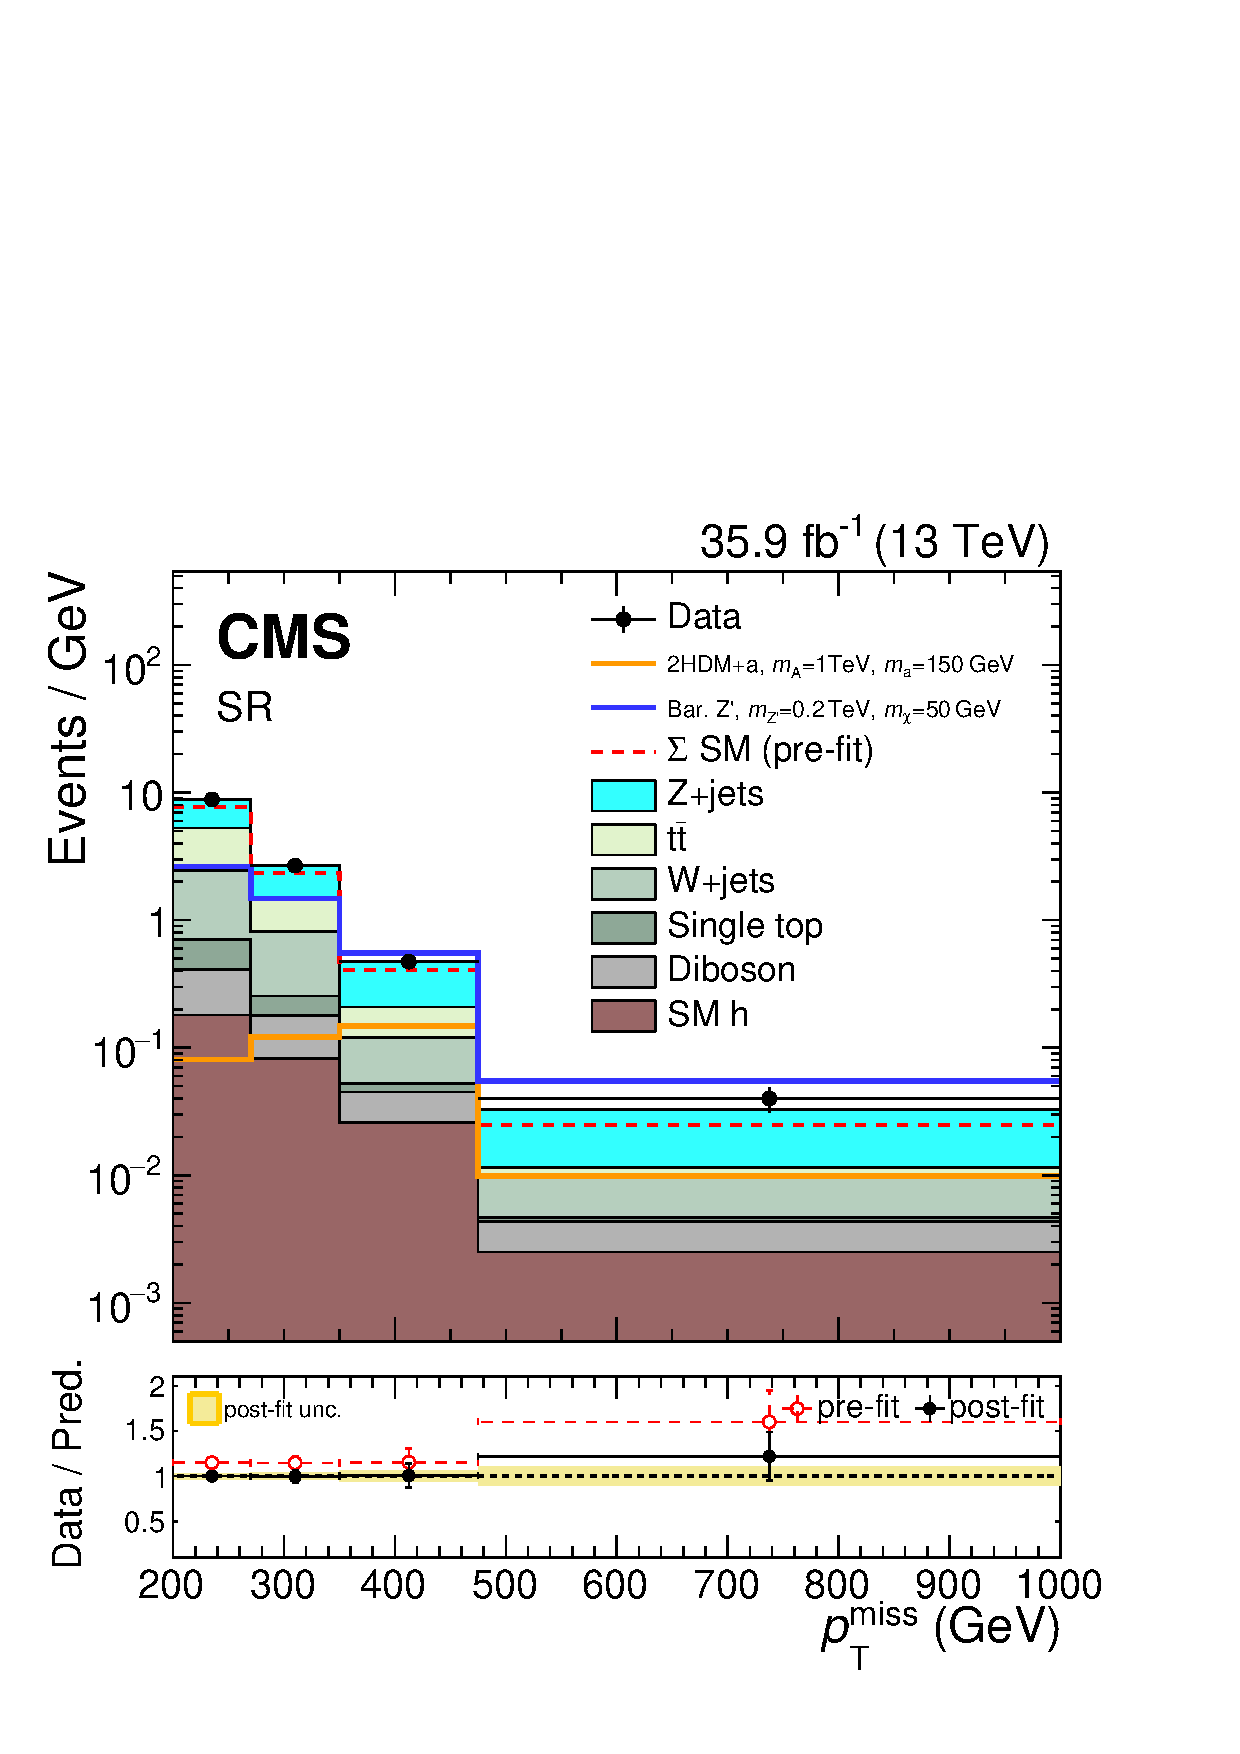
\includegraphics[width=0.4\textwidth]{figures/dataMC/MSDcorr_stackedPostfit_signal.pdf}} 
 \subfloat{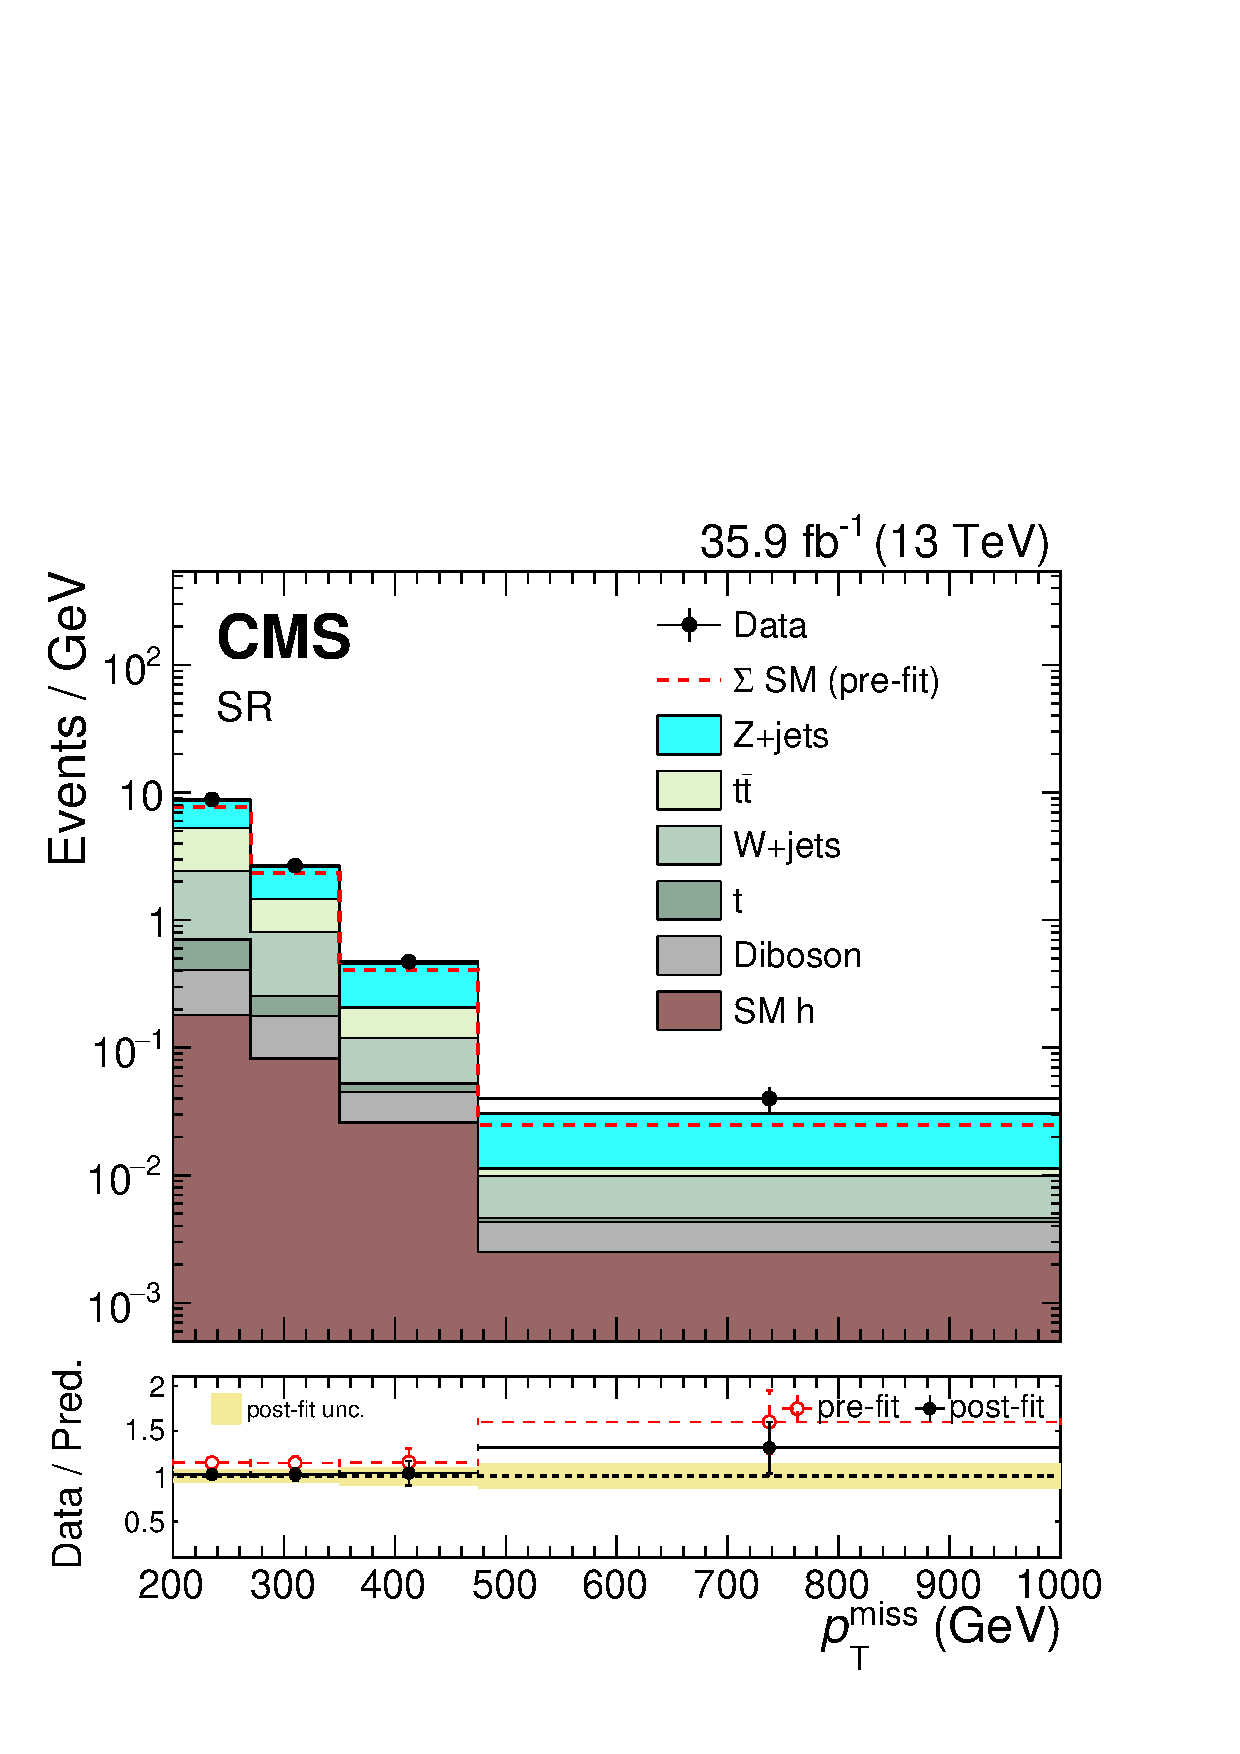
\includegraphics[width=0.4\textwidth]{figures/dataMC/MSDcorr_stackedPostfit_signal_masked.pdf}} \\
\caption{Shown is the \MET distribution in the signal region after a fit to data including the signal region (left) and excluding the signal region (right).}
\label{Fig_cr_Recoil_fail}
\end{figure}

%The different CRs defined in Table~\ref{tab:event_selection} are used to control the three main background processes.  Since the hadronic recoil $U$ is computed removing the muon(s) or the electron(s) from the \MET calculation, its distribution can be used as a proxy to model the \MET distribution in the SR. 
%Both the normalization and the shape of the \ttbar, Z+jets, and W+jets background processes are constrained by transfer factors from the CRs to the SR estimated in bins of $U$. These transfer factors correlate the same bins across all regions and are allowed to vary within uncertainties.% as described in Section~\ref{sec:systematics}.
To estimate the Z+jets production in the signal region, CRs enriched in dimuon and dielectron events are used.
Dimuon events are selected online employing the same \MET triggers that are used in the SR.
These events are required to have two opposite-charge muons (having a \pt greater than $20\GeV$ and $10\GeV$ for the leading and trailing muon, respectively), that form an invariant mass between 60\GeV and 120\GeV.
The leading muon also has to pass tight identification and isolation requirements.
%Events in the dimuon region must also pass almost all other selection requirements imposed on the events in the signal region, wherein $U$ is substituted for \ptmiss.
%In order to increase the number of events in the dimuon CR, the requirement of the fat jet b tag is not imposed.
Dielectron events are selected online using single electron triggers.%, which have a \pt threshold of $27\GeV$.
Two opposite-charge electrons with \pt greater than $10\GeV$ are required offline, and they must form an invariant mass between 60\GeV and 120\GeV.
To be on the plateau of the trigger efficiency, at least one of the two electrons must have $\pt>40\GeV$ and satisfy tight identification and isolation requirements.
%All selection criteria applied in the dimuon CR are applied in the dielectron CR.
Events that enter the signal selection due to the loss of a single lepton primarily arise from W+jets and semileptonic \ttbar events.
To estimate these backgrounds, four single-lepton samples are used: single muon and single electron, with or without an additional b-tagged AK4 jet.
The b-tagged single lepton CRs target \ttbar events, while the anti-b-tagged single lepton CRs target W+jets events.
Single muon events are selected using the \MET trigger.
The muon candidate in these events is required to have \pt greater than 20\GeV, and is required to be well identified and isolated.
%With the exception of b tagging, all other selection requirements used for signal events are imposed, using $U$ instead of \ptmiss.
In the b-tagged single muon CR, exactly one b-tagged AK4 jet non overlapping with the CA15 jet is required.
In the anti-b-tagged single muon CR, the b tagging requirement is reversed.
Each CR is split into two  subsamples depending on whether or
not they satisfy the same requirement on the output of double-b tagger imposed to define the SR. This allows for an {\it in situ} calibration of the scale factor that corrects the mis-identification probability of the double-b tagger for the three main backgrounds. 


The results are extracted with a binned liklihood fit (using the ROOStat package~\cite{roostats}) to the \MET and $U$ spectra. A simultaneous fit is performed on all the CRs and the SR. 
The dominant SM process in each CR is used to estimate at least one of the backgrounds in the SR. Each constraint is applied via a transfer factor $R$, which is ratio of the expected yield of the target process in the signal region and the expected yield of the process in the CR. $R$ is defined as a function of $U$ and estimated using simulation. 
If $b\ell$ is the subsample of the single lepton control sample that is used to estimate the \ttbar process in the SR, the free parameter $\mu^{\ttbar}_i$ will be included in the likelihood to represent the number of events observed in bin $i$ of $U$ in the SR. The expected number of events $N^{b\ell}_{i}$ is then given by $N^{b\ell}_{i}=  \dfrac{{\mu^{\ttbar}_{i}}}{R^{b\ell}_{i}}$.
The transfer factors $R^{\ell}$ and $R^{b\ell}$ used to constrain the W+jets and the $t\bar{t}$ background respectively are derived from simulation, taking into account the impact of lepton acceptances and efficiencies, the b-tagging efficiency, and, for the single electron control sample, the additional \MET requirement.
%This transfer factor explicitly includes hadronic tau leptons that fail the hadronic tau lepton identification criteria, which account for roughly 20-80\% of the total W+jets background in the high recoil region.  differences in \ptmiss trigger efficiencies observed between single-muon and dimuon events,
Because of a large \ttbar contamination in the W+jets pass CR, an additional transfer factor is imposed between the \ttbar in the b-tagged and anti-b-tagged single-lepton CRs.
%This allows for an estimation of the \ttbar contribution in the signal region to be made from W+jets CRs to be made from the b-tagged CR. 
A similar constraint is imposed to estimate the contamination from W+jets production in the $t\bar{t}$ CR composed by events that do not satisfy the requirement on the double-b output. 
The Z+jets background prediction in the signal region is connected to the dimuon and dielectron CRs through transfer factors ($R^{\ell\ell}$).
They are derived using simulation and account for the difference in the branching fractions of $\mathrm{Z}\rightarrow \nu\nu$~and $\mathrm{Z}\rightarrow \ell\ell$ decays and the impacts of lepton acceptances and selection efficiencies.

